

\documentclass{beamer}
\usetheme{Berlin}
\usecolortheme{default}

\usepackage{cmap}                   % поиск в PDF
\usepackage{braket}
\usepackage[T2A]{fontenc}           % кодировка
\usepackage{mathtext}               % русские буквы в формулах
\usepackage[utf8]{inputenc}         % кодировка исходного текста
\usepackage[english,russian]{babel} % локализация и переносы
\usepackage{multimedia}             % вставка видео
\setbeamertemplate{caption}[numbered] % нумерование иллюстраций

\title{Реализация квантового компьютера на ионной ловушке}
\subtitle{Вопрос по выбору к ГКЭ, январь 2022}
\author{Станислав Сидельников Б01-908, Егор Батарин Б01-906}
\institute{Московский физико-технический институт}
\date{}


% TODO:
% 1) Добавить формулы DONE
% 2) Исправить и добавить описание процесса
%    Инициализации
% 3) Добавить описание измерений
% 4) Проверить всю презентацию на ошибки

\begin{document}
    
    \begin{frame}
        \titlepage
    \end{frame}

    \begin{frame}{Содержание}

        \begin{itemize}

            \item<1-> Введение в квантовые вычисления

      

            \item<2-> Принцип работы ионной ловушки

                \begin{itemize}
                    \item{Захват иона}
                    \item{Доплеровское охлаждение}
                    \item{Pro \& Contra}
                \end{itemize}

            \item<3-> Кубит на ионной ловушке

                \begin{itemize}


                    \item{Физическая реализация кубита}
                    \item{Приготовление начального состояния}
                    \item{Измерение конечного результата}

                \end{itemize}
            
            \end{itemize}

                
        \end{frame}

	\begin{frame}
		\titlepage
	\end{frame}
	
	\begin{frame}{Содержание}
		
		\begin{itemize}
			
			\item<1-> Введение в квантовые вычисления
			
			
			
			\item<2-> Принцип работы ионной ловушки
			
			\begin{itemize}
				\item{Захват иона}
				\item{Доплеровское охлаждение}
				\item{Pro \& Contra}
			\end{itemize}
			
			\item<3-> Кубит на ионной ловушке
			
			\begin{itemize}
				
				
				\item{Физическая реализация кубита}
				\item{Приготовление начального состояния}
				\item{Оптическая накачка}
				\item{Измерение конечного результата}
				
			\end{itemize}
			
		\end{itemize}
		
		
	\end{frame}
	
	\begin{frame}{Введение в квантовые вычисления}
		Классический бит: $0$ или $1$ - два состояния.
		\vspace{3mm}
		
		Квантовый бит: $\ket{\psi} = \alpha\ket{0} + \beta\ket{1}$, $\alpha,\beta \in \mathbb{C}$, $|\alpha|^2 + |\beta|^2 = 1$ - бесконечно много состояний?
		\vspace{3mm}
		
		Представление на сфере Блоха: $\ket{\psi} = e^{i\gamma}\left(  \cos{\frac{\theta}{2}}\ket{0}+e^{i\phi}\sin{\frac{\theta}{2}} \ket{1}  \right) \sim \cos{\frac{\theta}{2}}\ket{0}+e^{i\phi}\sin{\frac{\theta}{2}} \ket{1} $,
		
		где $\gamma, \theta$ и $\phi$ - действительные числа.
	\end{frame}
	
	\begin{frame}{Введение в квантовые вычисления}
		
		\begin{figure}[]
			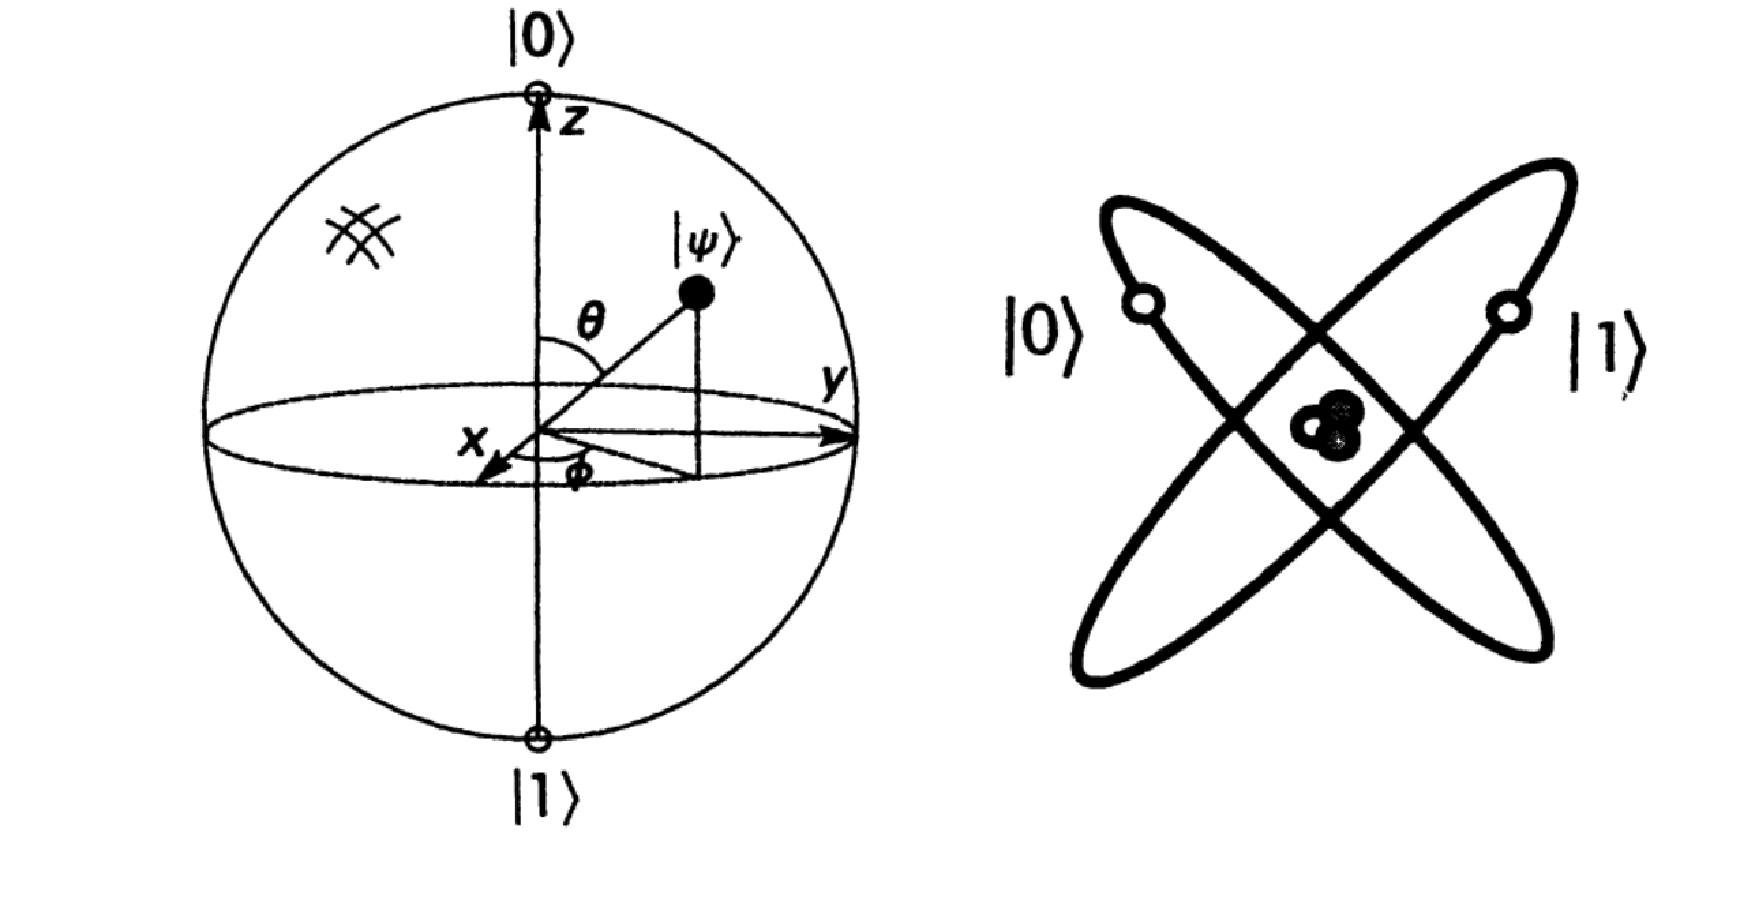
\includegraphics[width=\linewidth]{media/qubits.pdf}
		\end{figure}
	\end{frame}

    \begin{frame}{Захват ионов}
    \framesubtitle{Принцип работы ионной ловушки}

        \begin{columns}

        \begin{column}{0.6\textwidth}

            \begin{itemize}
                \item Между внутренним и внешним участками каждого электрода поддерживается
                разность потенциалов $U_{0}$, так что ионы находятся в статическом потенциале
                $\varphi_{static} = k U_{0} [\ z^2 - (x^2 + y^2) ]\ $
                \item По \textit{теореме Ирншоу} заряд не может находится в положении устойчивого равновесия
            \end{itemize}

        \end{column}

        \begin{column}{0.5\textwidth}
            \begin{figure}
                \centering
                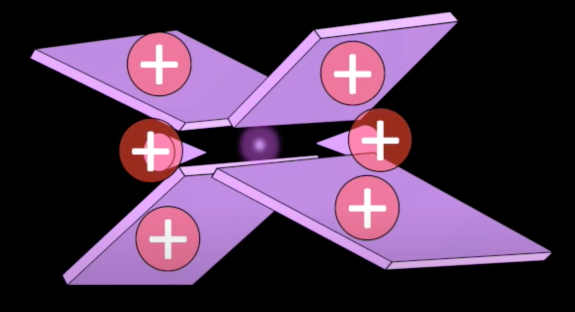
\includegraphics[width=\textwidth]{media/ion-trap.png}
                \caption{Схема ионной ловушки}
            \end{figure}
        \end{column}

        \end{columns}

    \end{frame}
	
	\begin{frame}{Захват ионов}
		\framesubtitle{Принцип работы ионной ловушки}
		
		\begin{columns}
			
			\begin{column}{0.5\textwidth}
				
				\begin{itemize}
					\only<1>{\item Мы рассматриваем ловушку Пауля. Данный тип ионной ловушки представляет собой систему электродов, между которыми находятся ионы.}
					\item<2-> Для содержания ионов в замкнутой области пространства используется
					периодическая смена напряжения электрического поля на обоих электродах:

					$E_x = - \frac{U + V \cos{\omega t}}{r_{0}^2} x$
					$E_z = \frac{U + V \cos{\omega t}}{r_{0}^2} z$
					$E_y = 0$

					\item<2-> $U$ - постоянное напряжение, $V$ - напряжение на частоте $\omega$
				\end{itemize}
				
			\end{column}
			
			\begin{column}{0.5\textwidth}
				\begin{figure}
					\centering
					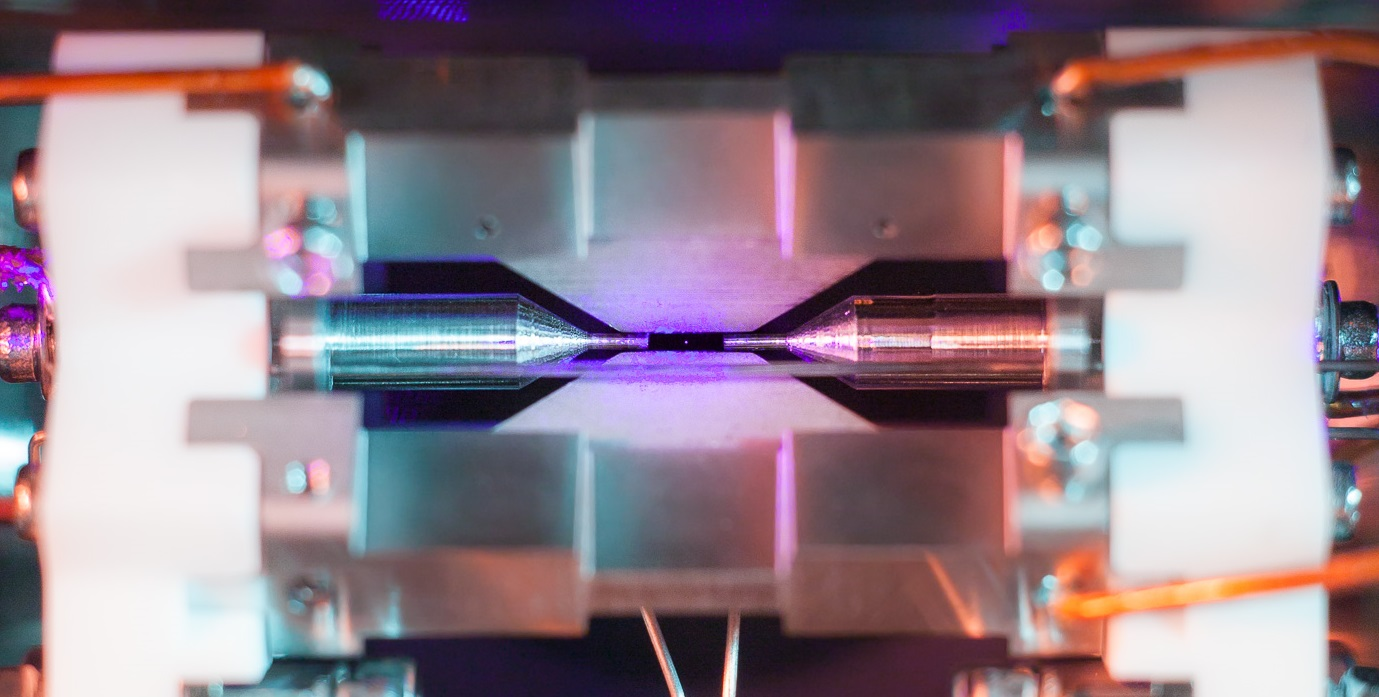
\includegraphics[width=\textwidth]{media/trapped-ion.jpg}
					\caption{Захваченный ион}
				\end{figure}
			\end{column}
			
		\end{columns}
	\end{frame}
	
	
	
	\begin{frame}{Захват ионов}
		\framesubtitle{Принцип работы ионной ловушки}
		
		\begin{columns}
			
			\begin{column}{0.5\textwidth}
				
				\begin{itemize}
					\only<1>{\item Получаем эффект динамической стабилизации: потенциал в ловушке представляет собой геометрически поверхность седла.}
					\only<2>{\item В статике положение равновесие шарика (механический аналог иона) в этом седле будет неустойчиво.}
					\only<2>{ В то время как если систему вращать вокруг оси, проходящей через центр седла перпендикулярно плоскости $xy$, то система
					будет устойчива.}
                    \only<3>{\item Получаем дифференциальных уравнений движения:
                    \[\ddot x + \frac{e}{m r_{0}^{2}}(\ U + V \cos{\omega t})\ x = 0 \]
                    \[\ddot z - \frac{e}{m r_{0}^{2}}(\ U + V \cos{\omega t})\ z = 0 \]}

                    \only<4>{\item Решением системы будут так называемые \textbf{Уравнения Матье}}
                    \only<4>{\item Уравнения Матье имеют два типа решений: устойчивое и неустойчивое движение. Существуют такие изменения U и V, что решением уравнений будет устойчивое движение.}

				\end{itemize}
				
			\end{column}
			
			\begin{column}{0.5\textwidth}
				\begin{figure}
					\centering
					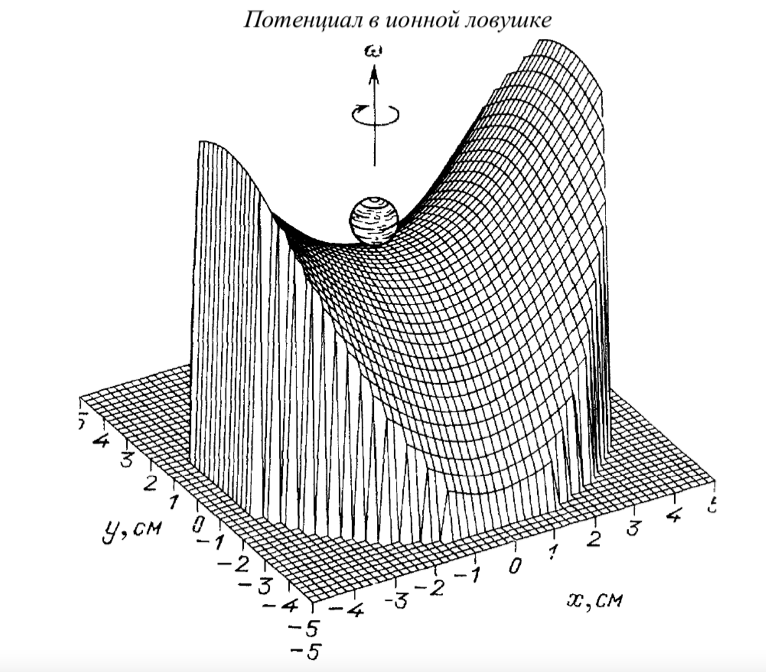
\includegraphics[width=\textwidth]{media/trap-potential.png}
					\caption{Захваченный ион}
				\end{figure}
			\end{column}
			
		\end{columns}
		
	\end{frame}



    \begin{frame}{Доплеровское охлаждение}
    \framesubtitle{Принцип работы ионной ловушки}

        \begin{columns}

        \begin{column}{0.5\textwidth}

            \begin{itemize}
                \item[1.] <1-> Покоящийся атом, смещения по частоте нет, налетающий фотон
                               не поглощается
                \item[2.] <2-> Атом движется. Смещение по частоте в область красного спектра,
                               поглощение фотона не происходит
                \item[3.1] <3-> Атом движется. Смещение по частоте в область синего спектра,
                                происходит поглощение фотона.
            \end{itemize}

        \end{column}

        \begin{column}{0.5\textwidth}
            \begin{figure}
                \centering
                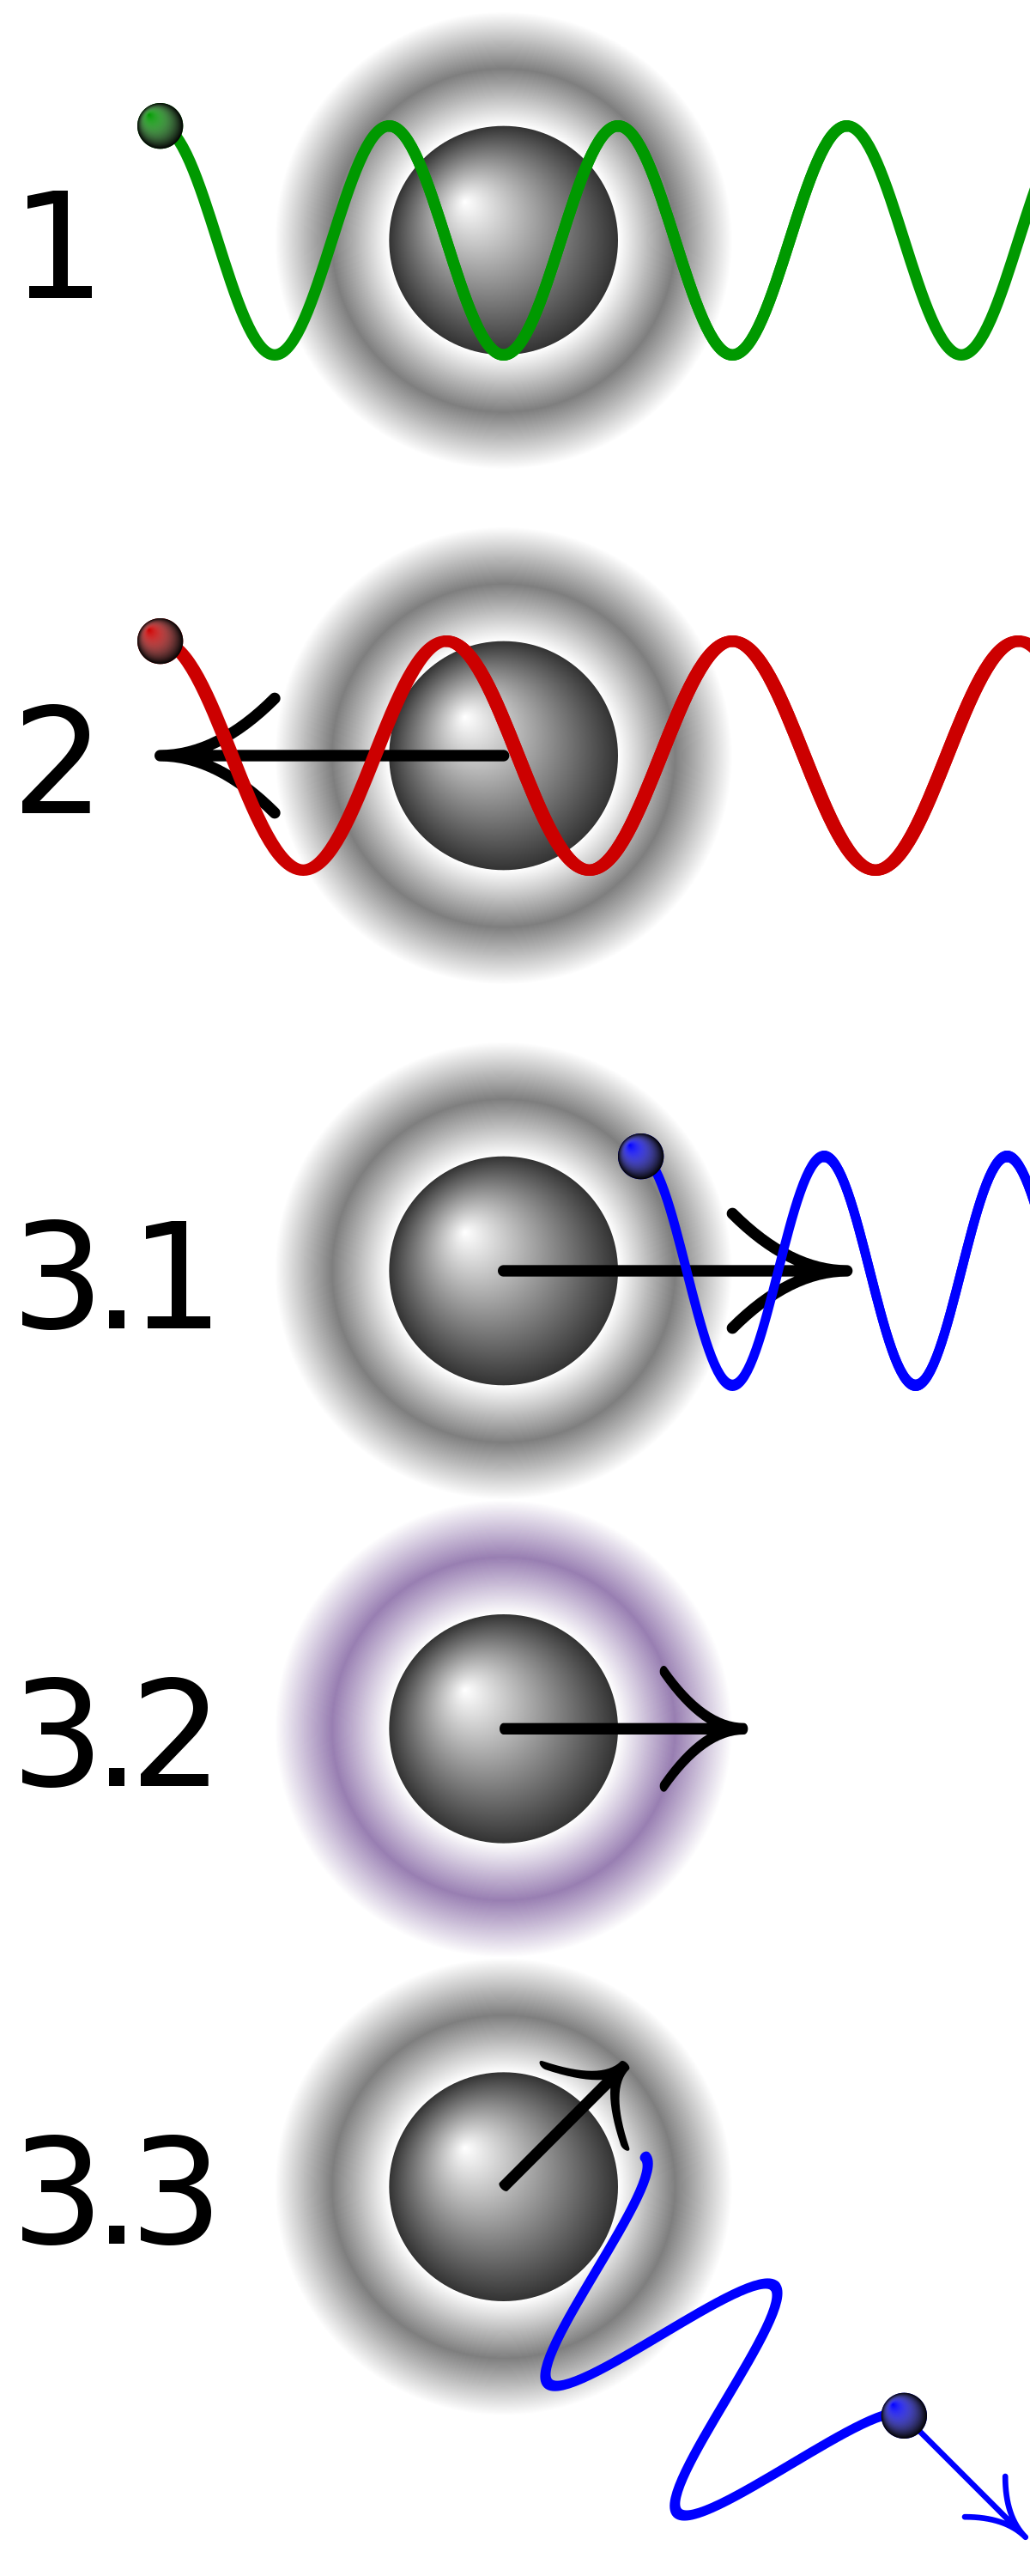
\includegraphics[width=0.35\textwidth]{media/dopler-cooling.png}
                \caption{Иллюстрация доплеровского охлаждения}
            \end{figure}
        \end{column}

        \end{columns}
    \end{frame}

    \begin{frame}{Доплеровское охлаждение}
    \framesubtitle{Принцип работы ионной ловушки}
        \begin{columns}

        \begin{column}{0.5\textwidth}

            \begin{itemize}
                \item[3.2] <1-> Атом возбуждается
                \item[3.3] <2-> Атом излучает в случайном направлении
            \end{itemize}

        \end{column}

        \begin{column}{0.5\textwidth}
            \begin{figure}
                \centering
                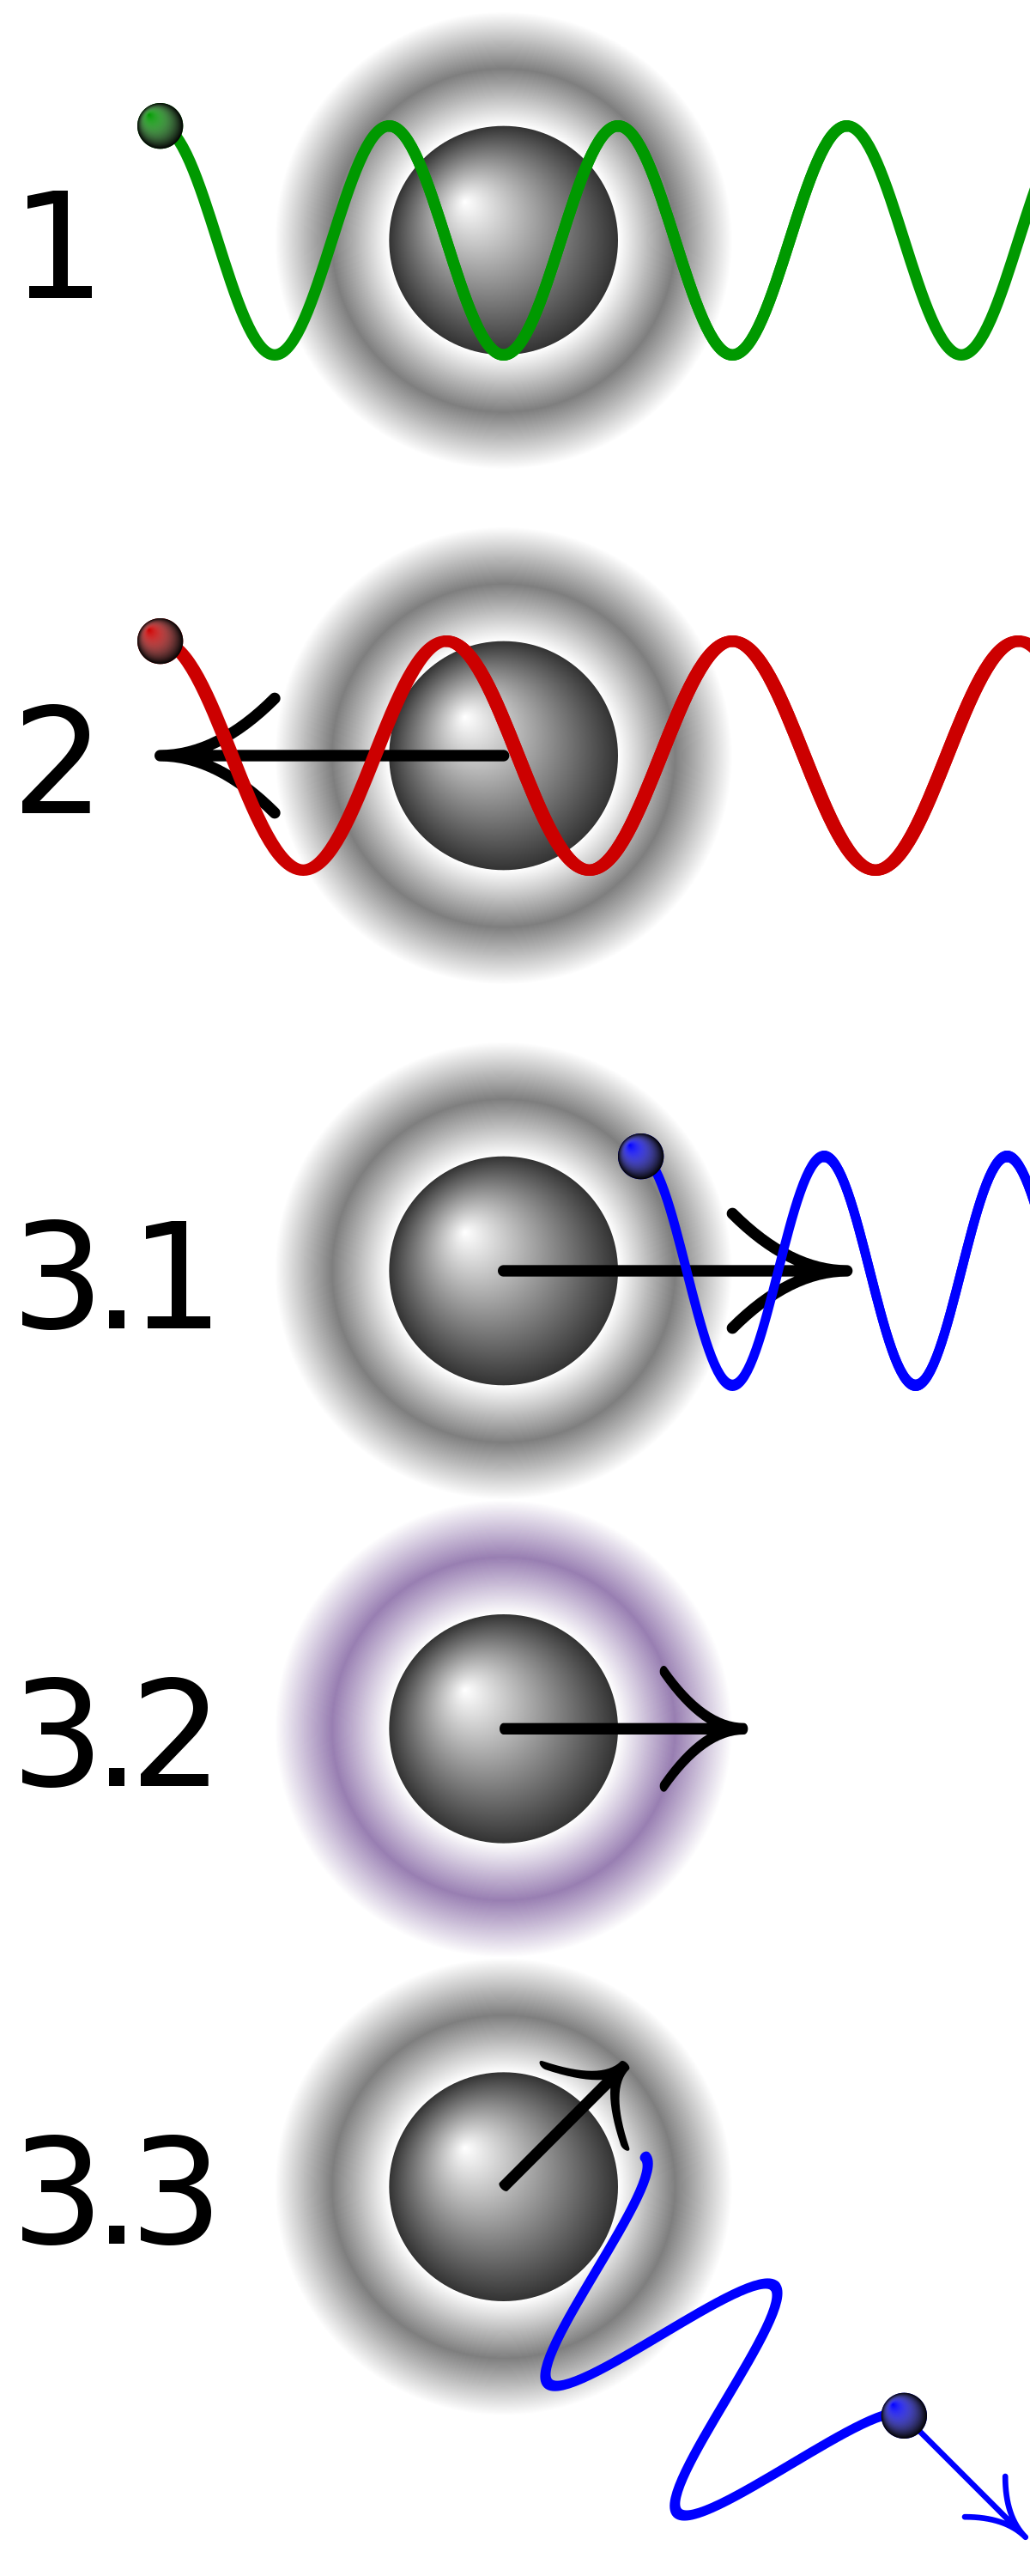
\includegraphics[width=0.35\textwidth]{media/dopler-cooling.png}
                \caption{Иллюстрация доплеровского охлаждения}
            \end{figure}
        \end{column}

        \end{columns}

    \end{frame}


    % \begin{frame}{Захват ионов}
    % \framesubtitle{Принцип работы ионной ловушки}

    %     \movie{\includegraphics[width=\textheight,
    %                      keepaspectratio]
    %                      {media/trapped-ion.jpg}}{media/paul-trap.mp4}

    % \end{frame}

    \begin{frame}{Физическая реализация кубита}
    \framesubtitle{Кубитная ионная ловушка}

        \begin{columns}

        \begin{column}{0.6\textwidth}

            \begin{itemize}
                \item <1-> Кубит представляет собой атомные состояния сверхтонкой структуры удерживаемых в ловушке атомов. 
                \item <2-> Два сверхтонких уровня основного состояния (они называются «сверхтонкими кубитами»)
                \item <3-> Уровень основного состояния и возбужденный уровень (они называются «оптическими кубитами»)
            \end{itemize}

        \end{column}

        \begin{column}{0.4\textwidth}
            \begin{figure}
                \centering
                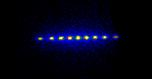
\includegraphics[width=\textwidth]{media/nine-calcium-ions.jpg}
                \caption{Девять атома кальция в ловушке}
            \end{figure}
        \end{column}

        \end{columns}

    \end{frame}

    \begin{frame}{Приготовление начального состояния}
    \framesubtitle{Кубитная ионная ловушка}

    \begin{itemize}
            \item <1-> Состояния ионных кубитов могут быть приготовлены в определенном состоянии кубита с помощью процесса, называемого \textbf{оптической накачкой}. В этом процессе лазер связывает ион с некоторыми возбужденными состояниями, которые в конечном итоге распадаются до одного состояния, которое не связано с лазером.
            \item <2-> Как только ион достигает этого состояния, у него нет возбужденных уровней, с которыми можно было бы взаимодействовать в присутствии этого лазера, и, следовательно, он остается в этом состоянии.
    \end{itemize}


    \end{frame}

    \begin{frame}{Приготовление начального состояния}
    \framesubtitle{Кубитная ионная ловушка}

    \begin{columns}

    \begin{column}{0.5\textwidth}

        \begin{itemize}
                \item <1-> Состояния ионных кубитов могут быть приготовлены в определенном состоянии кубита с помощью процесса, называемого \textbf{оптической накачкой}.
                \item <2-> Данный процесс
        \end{itemize}

    \end{column}

    \begin{column}{0.5\textwidth}

        \begin{figure}
            \centering
            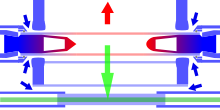
\includegraphics[width=\textwidth]{media/optical-pumping.png}
            \caption{Оптическая накачка лазерного стержня дуговой лампой}
        \end{figure}

    \end{column}

    \end{columns}


    \end{frame}

    \begin{frame}{Приготовление начального состояния}
    \framesubtitle{Кубитная ионная ловушка}

    \begin{itemize}
            \item <1-> Если ион распадается до одного из других состояний, лазер будет продолжать возбуждать ион до тех пор, пока он не распадется до состояния, которое не взаимодействует с лазером. Этот процесс инициализации является стандартным для многих физических экспериментов и может выполняться с очень высокой точностью (> 99,9)
    \end{itemize}

    \end{frame}


    \begin{frame}{Измерение состояния}

    \end{frame}



\end{document}

	
	\begin{frame}{Доплеровское охлаждение}
		\framesubtitle{Принцип работы ионной ловушки}
		
		\begin{columns}
			
			\begin{column}{0.5\textwidth}
				
				\begin{itemize}
					\item[1.] <1-> Покоящийся атом, смещения по частоте нет, налетающий фотон
					не поглощается
					\item[2.] <2-> Атом движется. Смещение по частоте в область красного спектра,
					поглощение фотона не происходит
					\item[3.1] <3-> Атом движется. Смещение по частоте в область синего спектра,
					происходит поглощение фотона.
				\end{itemize}
				
			\end{column}
			
			\begin{column}{0.5\textwidth}
				\begin{figure}
					\centering
					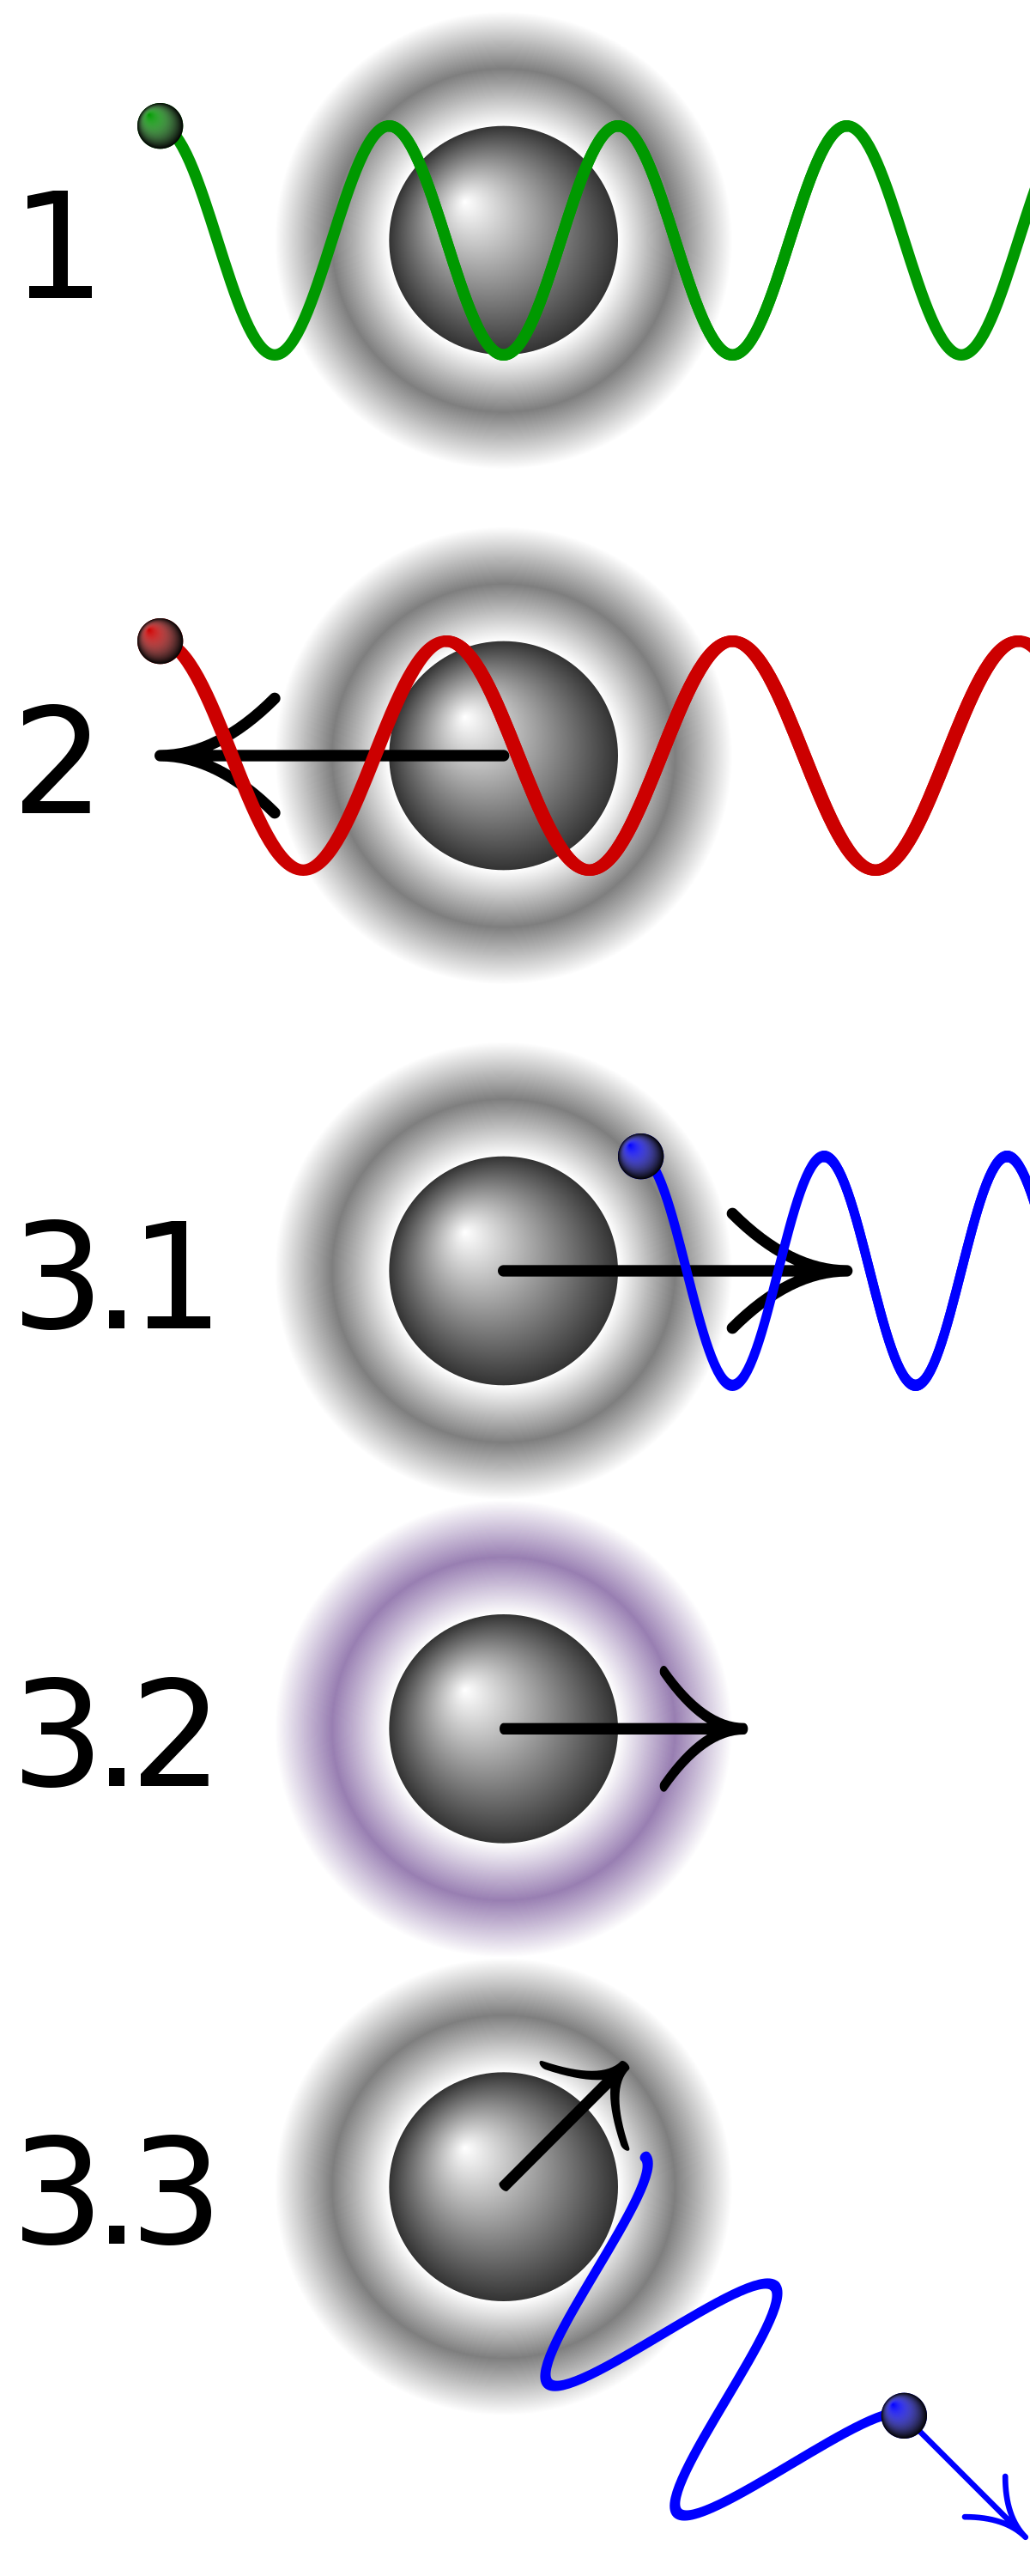
\includegraphics[width=0.35\textwidth]{media/dopler-cooling.png}
					\caption{Иллюстрация доплеровского охлаждения}
				\end{figure}
			\end{column}
			
		\end{columns}
	\end{frame}
	
	\begin{frame}{Доплеровское охлаждение}
		\framesubtitle{Принцип работы ионной ловушки}
		\begin{columns}
			
			\begin{column}{0.5\textwidth}
				
				\begin{itemize}
					\item[3.2] <1-> Атом возбуждается
					\item[3.3] <2-> Атом излучает в случайном направлении
				\end{itemize}
				
			\end{column}
			
			\begin{column}{0.5\textwidth}
				\begin{figure}
					\centering
					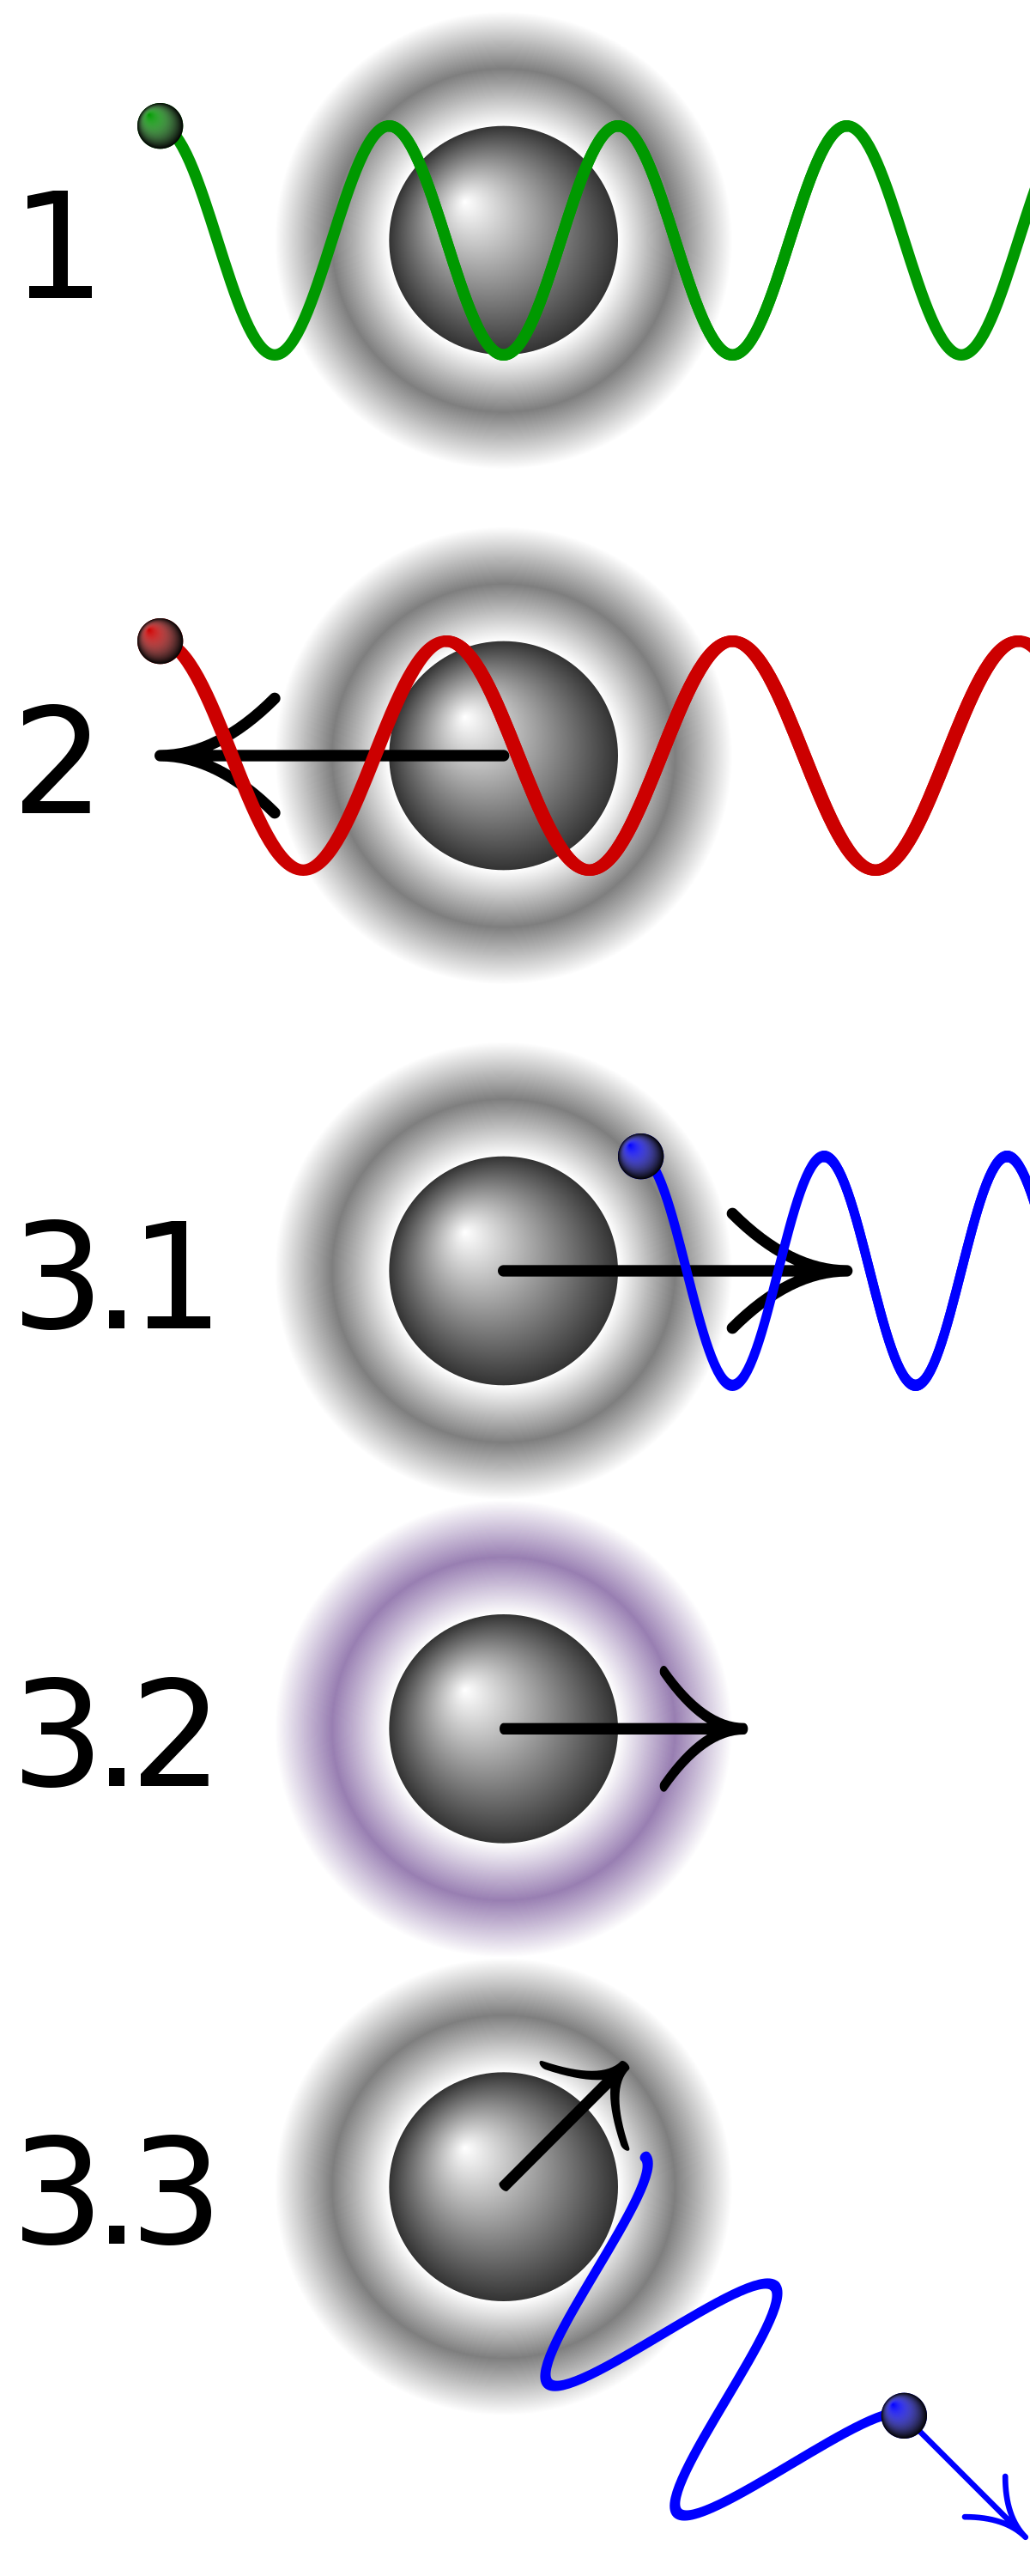
\includegraphics[width=0.35\textwidth]{media/dopler-cooling.png}
					\caption{Иллюстрация доплеровского охлаждения}
				\end{figure}
			\end{column}
			
		\end{columns}
		
	\end{frame}
	
	
	% \begin{frame}{Захват ионов}
	% \framesubtitle{Принцип работы ионной ловушки}
	
	%     \movie{\includegraphics[width=\textheight,
	%                      keepaspectratio]
	%                      {media/trapped-ion.jpg}}{media/paul-trap.mp4}
	
	% \end{frame}
	
	\begin{frame}{Физическая реализация кубита}
		\framesubtitle{Кубитная ионная ловушка}
		
		\begin{columns}
			
			\begin{column}{0.6\textwidth}
				
				\begin{itemize}
					\item  Кубит представляет собой атомные состояния сверхтонкой структуры удерживаемых в ловушке атомов. 
					\item  Два сверхтонких уровня основного состояния (они называются «сверхтонкими кубитами»)
					\item  Уровень основного состояния и возбужденный уровень (они называются «оптическими кубитами»)
				\end{itemize}
				
			\end{column}
			
			\begin{column}{0.4\textwidth}
				\begin{figure}
					\centering
					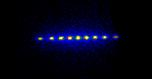
\includegraphics[width=\textwidth]{media/nine-calcium-ions.jpg}
					\caption{Девять атома кальция в ловушке}
				\end{figure}
			\end{column}
			
		\end{columns}
	\end{frame}
	
	\begin{frame}{Приготовление начального состояния}
		\framesubtitle{Кубитная ионная ловушка}
		
		\begin{itemize}
			\item <1-> Состояния ионных кубитов могут быть приготовлены в определенном состоянии кубита с помощью процесса, называемого \textbf{оптической накачкой}. В этом процессе лазер связывает ион с некоторыми возбужденными состояниями, которые в конечном итоге распадаются до одного состояния, которое не связано с лазером.
			\item <2-> Как только ион достигает этого состояния, у него нет возбужденных уровней, с которыми можно было бы взаимодействовать в присутствии этого лазера, и, следовательно, он остается в этом состоянии.
		\end{itemize}
		
		
	\end{frame}
	
	\begin{frame}{Приготовление начального состояния}
		\framesubtitle{Кубитная ионная ловушка}
		
		\begin{itemize}
			\item <1-> Если ион распадается до одного из других состояний, лазер будет продолжать возбуждать ион до тех пор, пока он не распадется до состояния, которое не взаимодействует с лазером. Этот процесс инициализации является стандартным для многих физических экспериментов и может выполняться с очень высокой точностью (> 99,9)
		\end{itemize}
		
	\end{frame}
	
	\begin{frame}{Оптическая накачка}
		\framesubtitle{Кубитная ионная ловушка}
		
		\begin{columns}
			
			\begin{column}{0.5\textwidth}
				
				\begin{itemize}
					\item 
				\end{itemize}
				
			\end{column}
			
			\begin{column}{0.5\textwidth}
				
				\begin{figure}
					\centering
					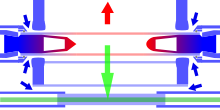
\includegraphics[width=\textwidth]{media/optical-pumping.png}
					\caption{Оптическая накачка лазерного стержня дуговой лампой}
				\end{figure}
				
			\end{column}
			
		\end{columns}
		
	\end{frame}
	
	\begin{frame}{Измерение состояния}
		
	\end{frame}
	
	
	
\end{document}

=======
	\end{frame}

    \begin{frame}{Принцип работы ионной ловушки}
    \framesubtitle{Доплеровское охлаждение}


        \begin{columns}

        \begin{column}{0.5\textwidth}

            \begin{itemize}
                \only<1>{\item Мы рассматриваем ловушку Пауля. Данный тип ионной ловушки представляет собой систему электродов, между которыми находятся ионы.}
                \item<2-> Для содержания ионов в замкнутой области пространства используется
                      периодическая смена напряжения электрического поля на обоих электродах:
                      $E_x = - \frac{U + V \cos{\omega t}}{r_{0}^2} x$,
                      $E_z = \frac{U + V \cos{\omega t}}{r_{0}^2} z$
                      $E_y = 0$
                \item<2-> $U$ - постоянное напряжение, $V$ - напряжение на частоте $\omega$
            \end{itemize}

        \end{column}

        \begin{column}{0.5\textwidth}
            \begin{figure}
                \centering
                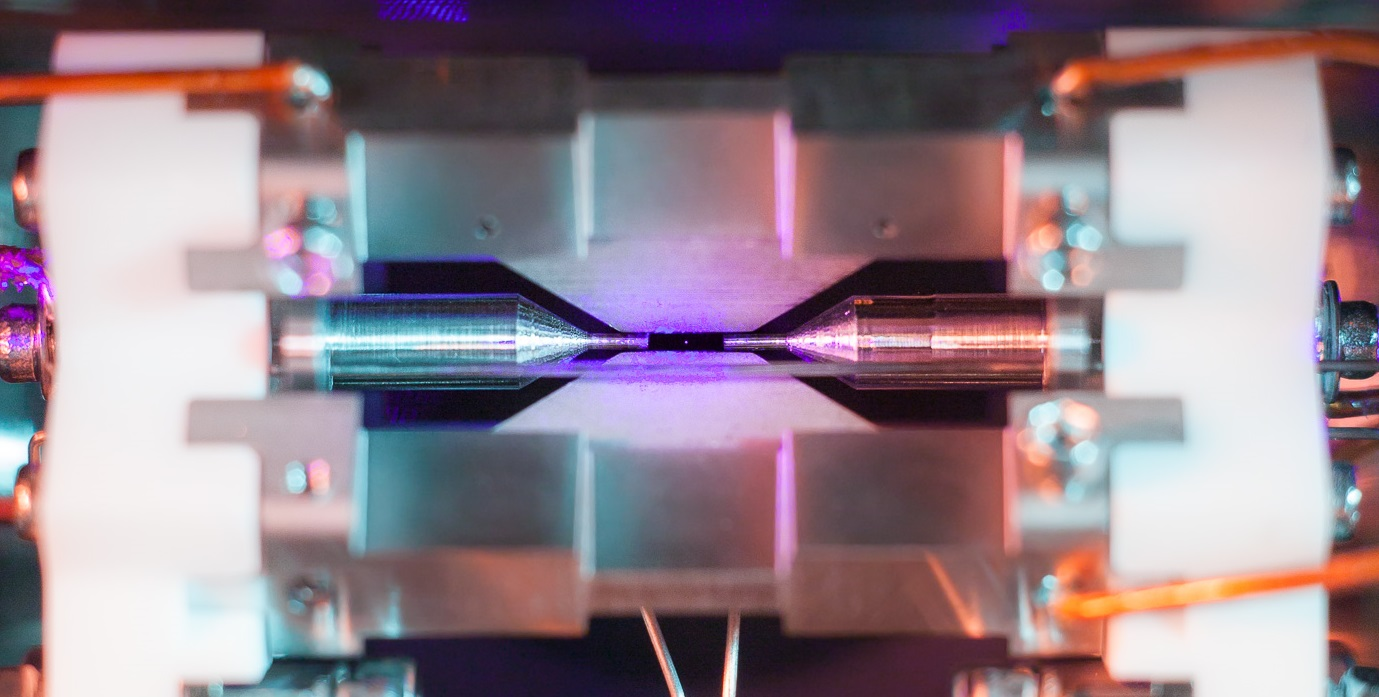
\includegraphics[width=\textwidth]{media/trapped-ion.jpg}
                \caption{Захваченный ион}
            \end{figure}
        \end{column}

        \end{columns}
    \end{frame}



    \begin{frame}{Захват ионов}
    \framesubtitle{Принцип работы ионной ловушки}

        \begin{columns}

        \begin{column}{0.5\textwidth}

            \begin{itemize}
                \only<1>{\item Получаем эффект динамической стабилизации: потенциал в ловушке представляет собой геометрически поверхность седла.}
                \item<2-> В статике положение равновесие шарика (механический аналог иона) в этом седле будет неустойчиво.
                \item<2-> В то время как если систему вращать вокруг оси, проходящей через центр седла перпендикулярно плоскости $xy$, то система
                будет устойчива.
            \end{itemize}

        \end{column}

        \begin{column}{0.5\textwidth}
            \begin{figure}
                \centering
                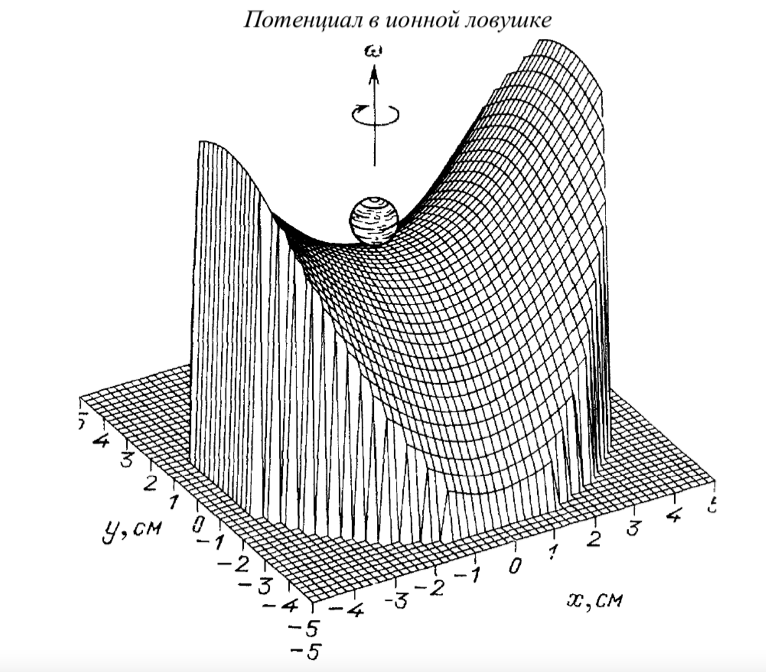
\includegraphics[width=\textwidth]{media/trap-potential.png}
                \caption{Захваченный ион}
            \end{figure}
        \end{column}

        \end{columns}

        \end{frame}


    \begin{frame}{Доплеровское охлаждение}
    \framesubtitle{Принцип работы ионной ловушки}

        \begin{columns}

        \begin{column}{0.5\textwidth}

            \begin{itemize}
                \item[1.] <1-> Покоящийся атом, смещения по частоте нет, налетающий фотон
                               не поглощается
                \item[2.] <2-> Атом движется. Смещение по частоте в область красного спектра,
                               поглощение фотона не происходит
                \item[3.1] <3-> Атом движется. Смещение по частоте в область синего спектра,
                                происходит поглощение фотона.
            \end{itemize}

        \end{column}

        \begin{column}{0.5\textwidth}
            \begin{figure}
                \centering
                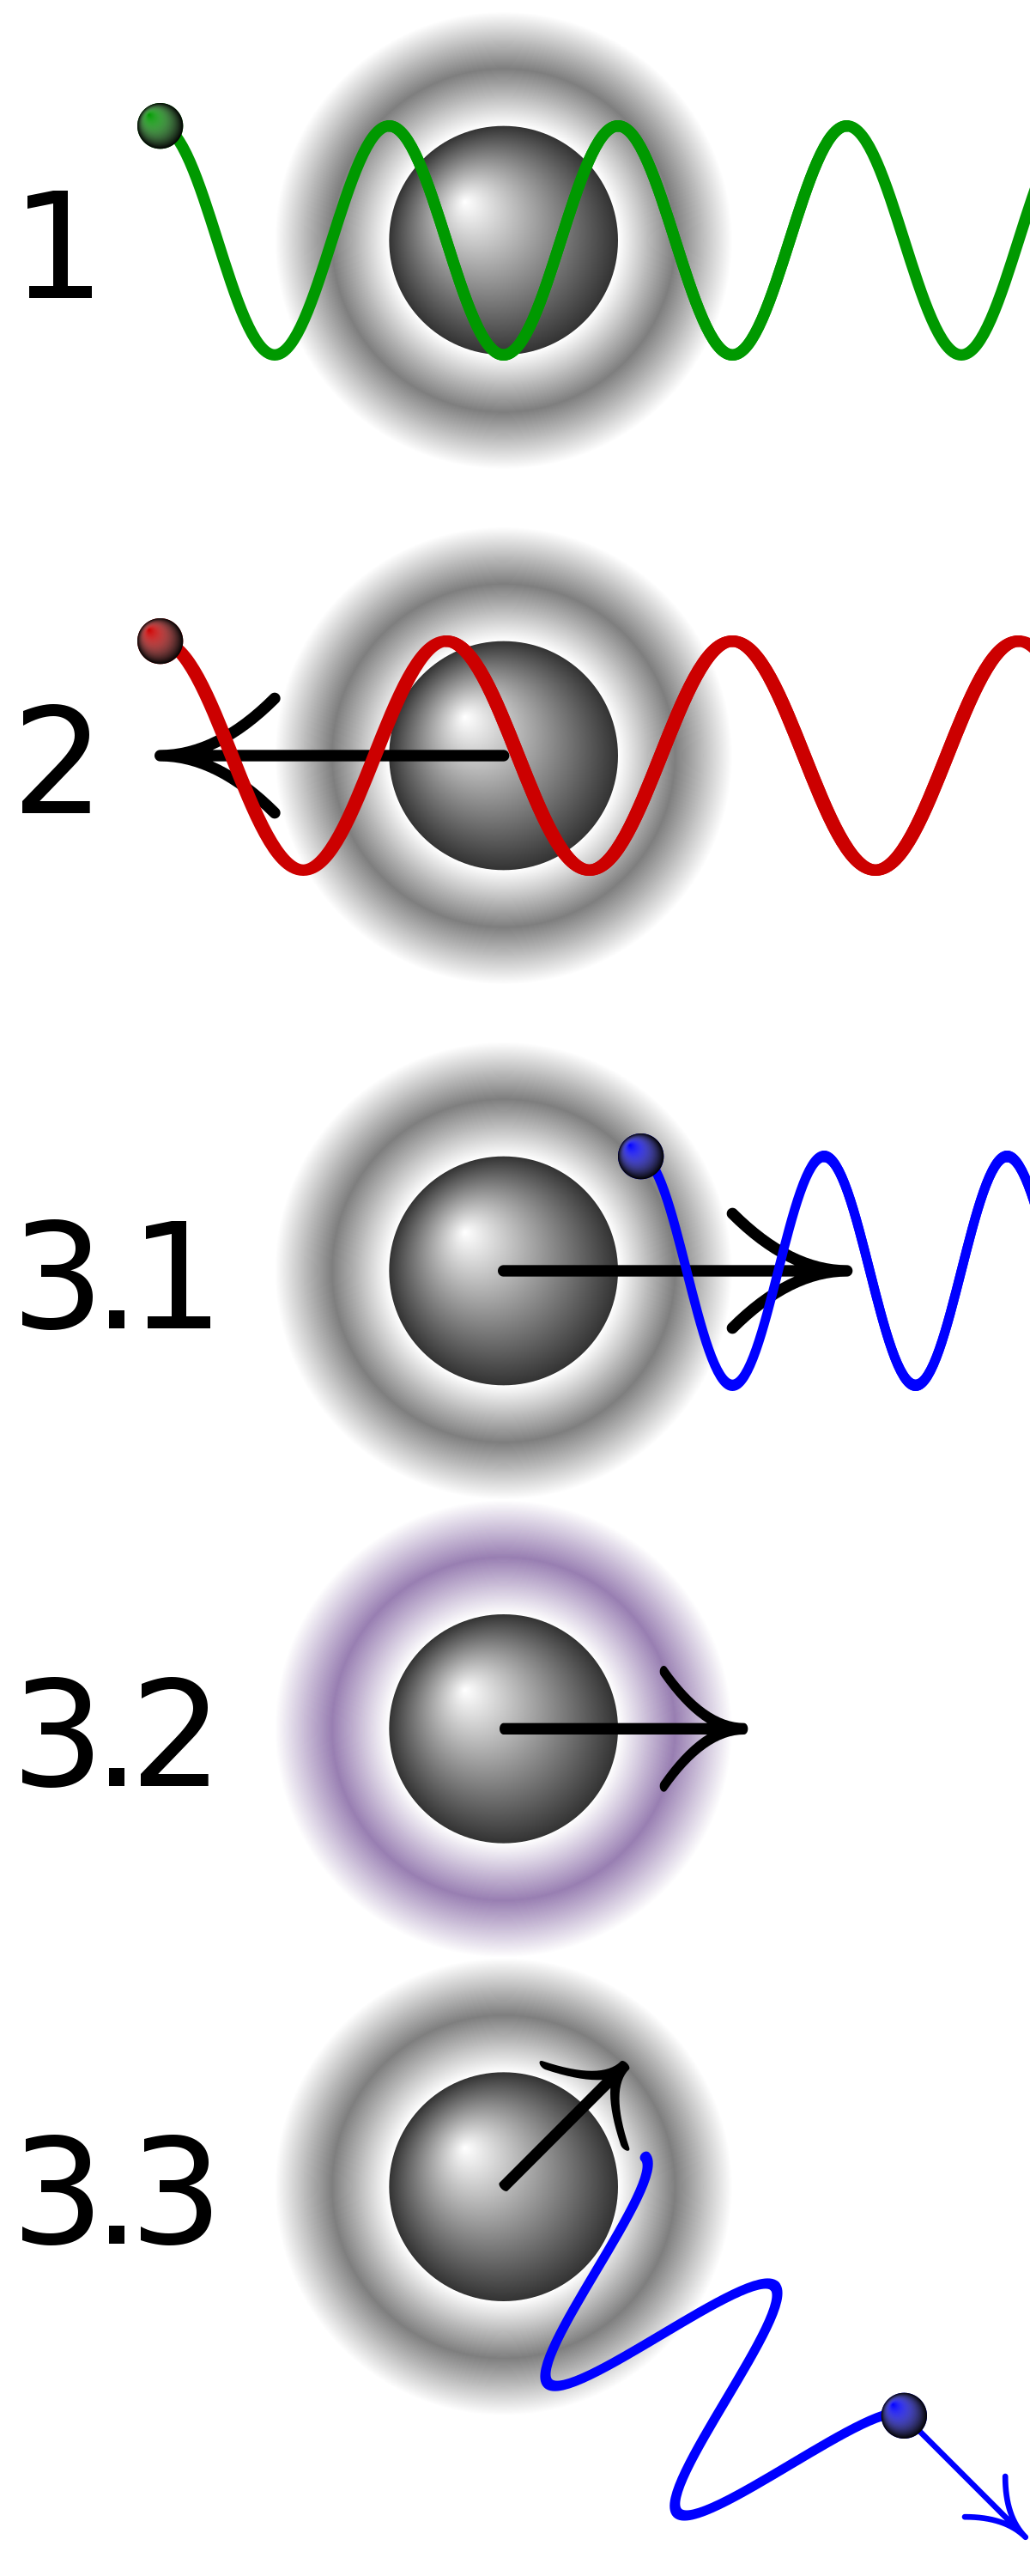
\includegraphics[width=0.35\textwidth]{media/dopler-cooling.png}
                \caption{Иллюстрация доплеровского охлаждения}
            \end{figure}
        \end{column}

        \end{columns}
    \end{frame}

    \begin{frame}{Доплеровское охлаждение}
    \framesubtitle{Принцип работы ионной ловушки}
        \begin{columns}

        \begin{column}{0.5\textwidth}

            \begin{itemize}
                \item[3.2] <1-> Атом возбуждается
                \item[3.3] <2-> Атом излучает в случайном направлении
            \end{itemize}

        \end{column}

        \begin{column}{0.5\textwidth}
            \begin{figure}
                \centering
                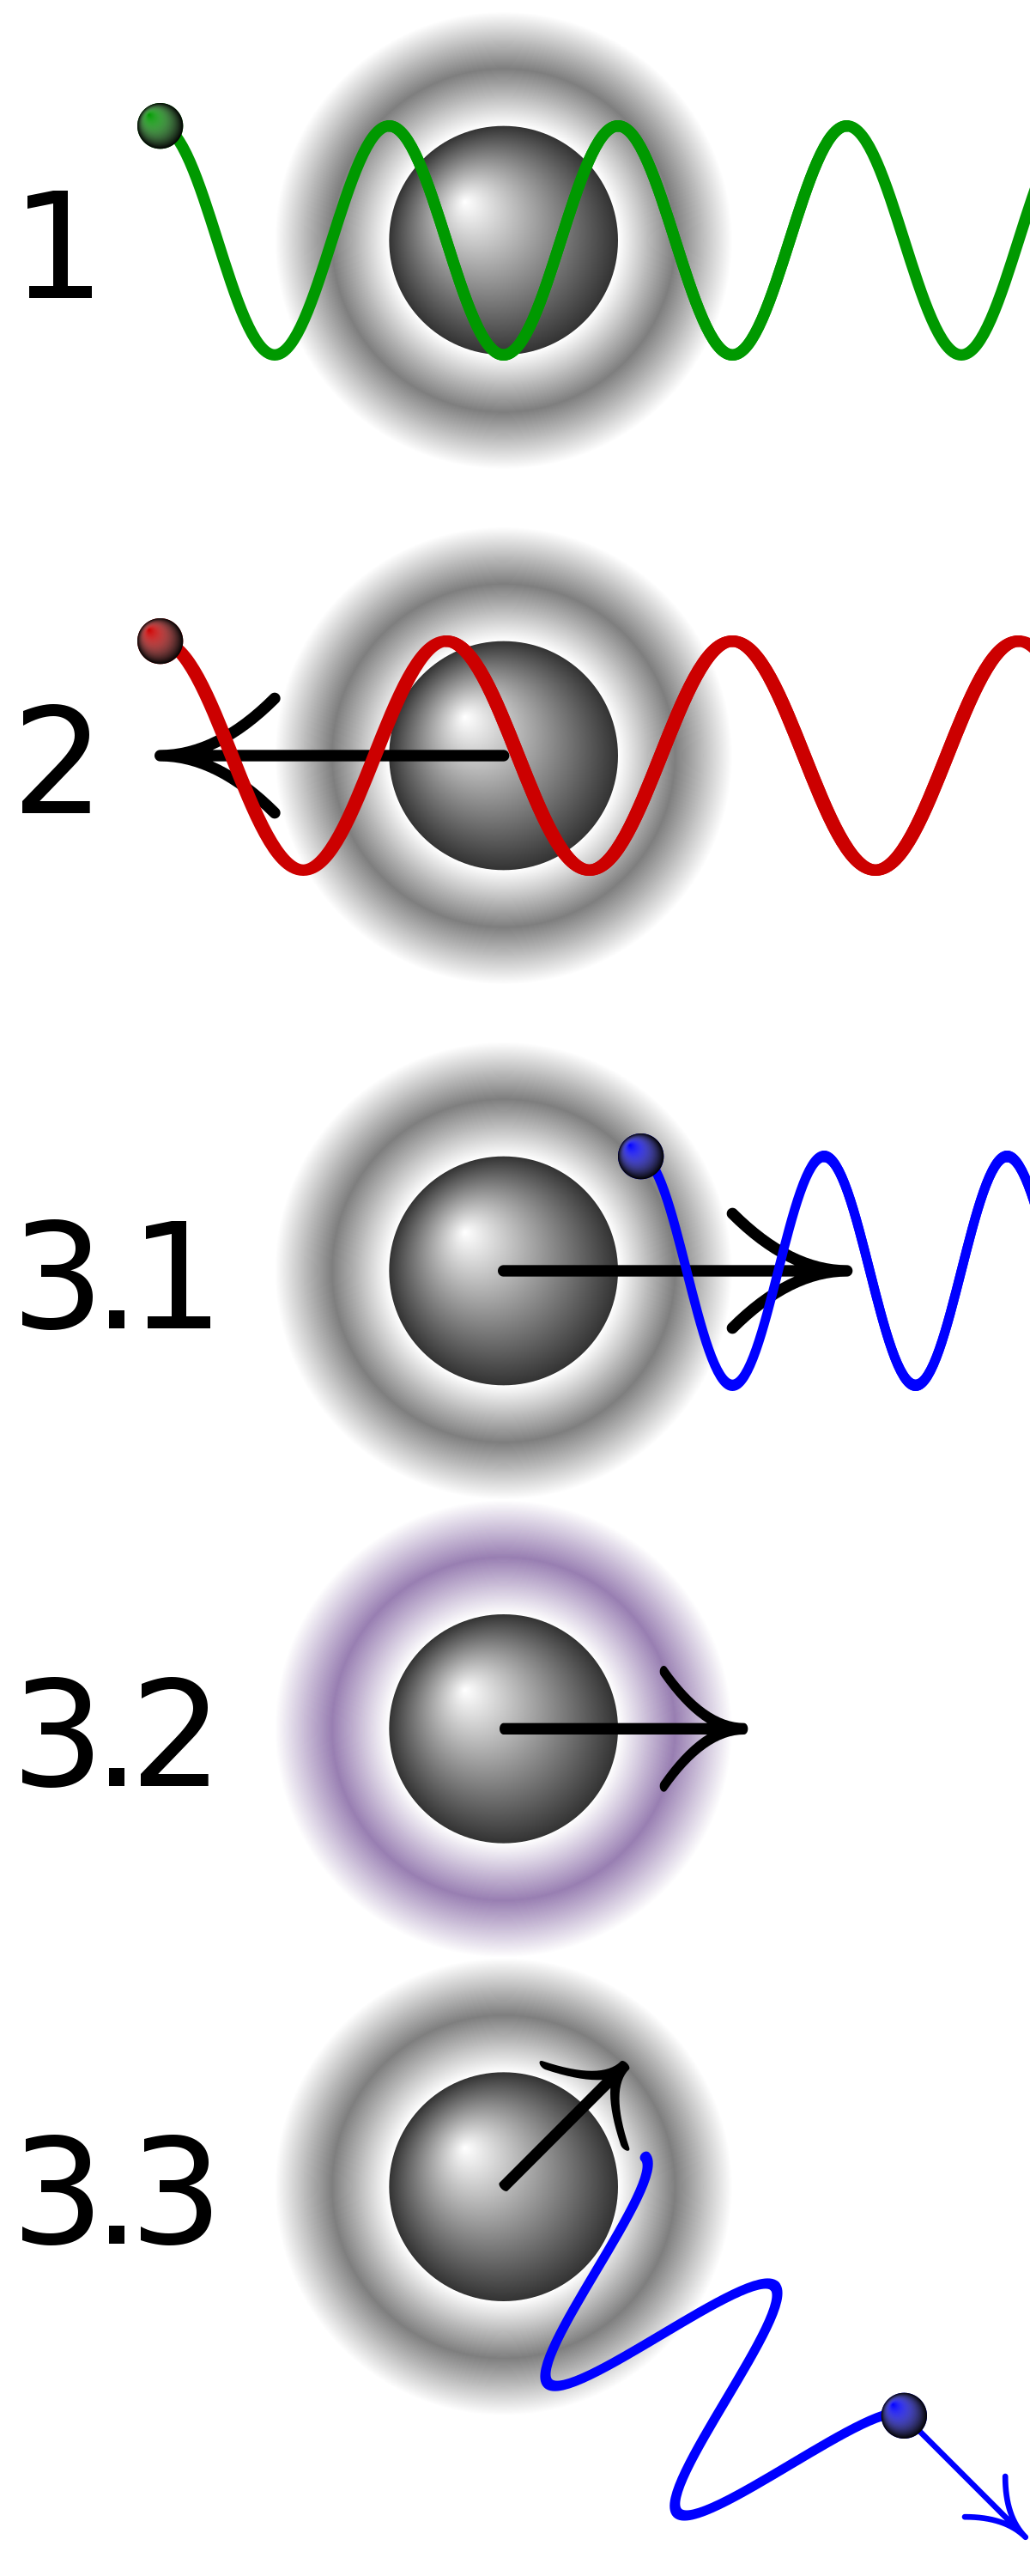
\includegraphics[width=0.35\textwidth]{media/dopler-cooling.png}
                \caption{Иллюстрация доплеровского охлаждения}
            \end{figure}
        \end{column}

        \end{columns}

    \end{frame}


    % \begin{frame}{Захват ионов}
    % \framesubtitle{Принцип работы ионной ловушки}

    %     \movie{\includegraphics[width=\textheight,
    %                      keepaspectratio]
    %                      {media/trapped-ion.jpg}}{media/paul-trap.mp4}

    % \end{frame}

    \begin{frame}{Физическая реализация кубита}
    \framesubtitle{Кубитная ионная ловушка}

        \begin{columns}

        \begin{column}{0.6\textwidth}

            \begin{itemize}
                \item <1-> Кубит представляет собой атомные состояния сверхтонкой структуры удерживаемых в ловушке атомов. 
                \item <2-> Два сверхтонких уровня основного состояния (они называются «сверхтонкими кубитами»)
                \item <3-> Уровень основного состояния и возбужденный уровень (они называются «оптическими кубитами»)
            \end{itemize}

        \end{column}

        \begin{column}{0.4\textwidth}
            \begin{figure}
                \centering
                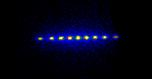
\includegraphics[width=\textwidth]{media/nine-calcium-ions.jpg}
                \caption{Девять атома кальция в ловушке}
            \end{figure}
        \end{column}

        \end{columns}

    \end{frame}

    \begin{frame}{Приготовление начального состояния}
    \framesubtitle{Кубитная ионная ловушка}

    \begin{columns}

    \begin{column}{0.5\textwidth}

        \begin{itemize}
                \item Ионизация вещества
                \item Заключение в ионную ловушку
                \item Доплеровское охлаждение
                \item Использование спонтанного и вынужденного излучения для
                      задание состояния иона
        \end{itemize}

    \end{column}

    \begin{column}{0.5\textwidth}

        \begin{figure}
            \centering
            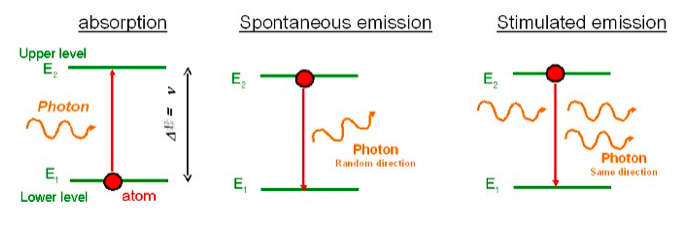
\includegraphics[width=\textwidth]{media/emission-comparison.png}
            \caption{Спонтанное и вынужденное излучение}
        \end{figure}

    \end{column}

    \end{columns}


    \end{frame}

    \begin{frame}{Приготовление начального состояния}
    \framesubtitle{Кубитная ионная ловушка}

    \begin{columns}

    \begin{column}{0.5\textwidth}

        \begin{itemize}
                \item Рассмотрим энергетические переходы в ионе кальция
                \item Учитывая, что времена жизни должны быть порядка микросекунд
                      для совершения квантовых операций, получим, что некоторые состояния
                      не годятся для выбора в качестве состояния $\ket{1}$
        \end{itemize}

    \end{column}

    \begin{column}{0.5\textwidth}

        \begin{figure}
            \centering
            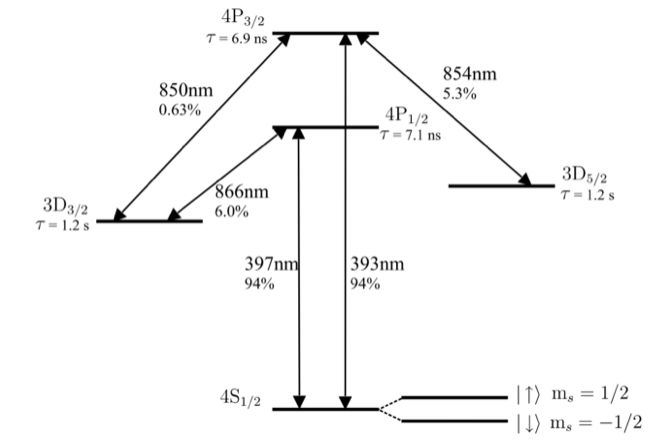
\includegraphics[width=\textwidth]{media/transitions.png}
            \caption{Спонтанное и вынужденное излучение}
        \end{figure}

    \end{column}

    \end{columns}


    \end{frame}


    \begin{frame}{Измерение состояния}

    \end{frame}

\end{document}
